% =====================================================================
% NegoPlay — FINAL PROJECT PORTFOLIO (תיק פרויקט)
% Structure per course submission guidelines:
%   p.1 title page · p.2 executive abstract (~200 words) ·
%   p.3 acknowledgments · p.4 table of contents · p.5+ full body
% Body = Part I Final Summary Report (incl. the requested AI-agents
% chapter and a software-engineering chapter) + Part II the full
% Preparatory Report (included PDF) + Part III the Business Plan
% (included PDF).
% Build: xelatex final_portfolio.tex (twice)
% =====================================================================
\documentclass[11pt, a4paper, oneside, openany]{report}

\usepackage[a4paper, margin=2.4cm]{geometry}
\usepackage{graphicx}
\usepackage{pdfpages}
\usepackage{booktabs}
\usepackage{tabularx}
\usepackage{enumitem}
\usepackage{float}
\usepackage{xcolor}
\usepackage{listings}
\usepackage{titlesec}
\usepackage[hidelinks]{hyperref}

\definecolor{navy}{HTML}{16324F}
\definecolor{steel}{HTML}{2C5F8A}
\definecolor{codebg}{HTML}{F4F6F8}

\titleformat{\chapter}[hang]{\bfseries\LARGE\color{navy}}{\thechapter\quad}{0pt}{}
\titlespacing*{\chapter}{0pt}{-20pt}{18pt}
\titleformat{\section}{\bfseries\Large\color{steel}}{\thesection\quad}{0pt}{}

\lstset{
  basicstyle=\ttfamily\footnotesize,
  backgroundcolor=\color{codebg},
  frame=single, framerule=0.3pt, rulecolor=\color{steel!40},
  breaklines=true, columns=fullflexible,
  keywordstyle=\bfseries\color{navy},
  commentstyle=\itshape\color{gray},
  language=Python, showstringspaces=false,
  xleftmargin=6pt, xrightmargin=6pt, aboveskip=8pt, belowskip=8pt
}

\begin{document}

% =====================================================================
% PAGE 1 — TITLE PAGE
% =====================================================================
\begin{titlepage}
\centering
\vspace*{1.8cm}
{\color{navy}\rule{\textwidth}{1.2pt}}\\[1.2cm]
{\Huge\bfseries\color{navy} NegoPlay\\[0.45cm]}
{\Large From Bridge Tables to the Negotiation Table:\\
Do Decision-Making Styles Transfer Across Domains?\\[1.0cm]}
{\color{navy}\rule{0.6\textwidth}{0.6pt}}\\[1.4cm]
{\large \textbf{Final Project Portfolio}\\
Final Summary Report \,\textperiodcentered\, Preparatory Report \,\textperiodcentered\, Business Plan\\[1.8cm]}
\begin{tabular}{rl}
\textbf{Submitted by:} & Anna Ben-Shushan \\[6pt]
\textbf{Course lecturer:} & Dr.\ Yoram Segal \\[6pt]
\textbf{PhD supervisor:} & Dr.\ Nezer Jacob Zaidenberg \\[6pt]
\textbf{Course:} & AI Development Expert \\[6pt]
\textbf{Institution:} & TESI --- The External Studies Institute \\[6pt]
\textbf{Submission date:} & June 14, 2026 \\
\end{tabular}\\[2.0cm]
{\color{navy}\rule{\textwidth}{1.2pt}}
\vfill
\end{titlepage}

% =====================================================================
% PAGE 2 — EXECUTIVE ABSTRACT (~200 words)
% =====================================================================
\chapter*{Executive Abstract}
\addcontentsline{toc}{chapter}{Executive Abstract}

Real-world negotiation data is proprietary and unmeasured, which makes
negotiation behaviour nearly impossible to study at scale. \textbf{NegoPlay}
uses competitive bridge as a measurable laboratory for the same decisions ---
risk, pressure, and information exchange --- and asks whether a player's
\emph{decision-making style} transfers from bridge to business negotiation.

From 149{,}208 tournament records (563 qualifying players), an unsupervised
pipeline discovered five statistically validated decision profiles
(Cohen's $d = 2.1$--$4.6$, all $p<0.05$). Each profile was converted into an
LLM agent whose system prompt contains only \emph{bridge-derived} skills, and
the agents negotiated business scenarios against a seller calibrated on
5{,}247 real Craigslist negotiations.

Win-rate transfer proved weak and metric-sensitive ($\rho \approx +0.2$);
refining the question to its original behavioural form showed that
\textbf{style transfers strongly}: bridge aggression and negotiation
aggression correlate at \textbf{Spearman $\rho = +0.80$}, above the
pre-registered $0.70$ target. An inverse-prompt control flips the correlation
to $-0.90$, proving the transfer is carried by the bridge-derived skills
rather than profile labels. The bridge metric itself was validated with a
random-baseline (``monkey'') test and a double-dummy evaluator. The system is
fully reproducible: a single SDK entry point, $100{+}$ unit tests, seeded
simulations, and per-call cost logging (total LLM spend ${\approx}\$1.70$).

% =====================================================================
% PAGE 3 — ACKNOWLEDGMENTS
% =====================================================================
\clearpage
\chapter*{Acknowledgments}
\addcontentsline{toc}{chapter}{Acknowledgments}

\vspace{0.5cm}
I would like to thank the people who accompanied this project from idea to
working system.

\vspace{0.4cm}
\textbf{Dr.\ Yoram Segal}, for the engineering-first project framework that
shaped this work --- the single-SDK discipline, the insistence on measurable
deliverables, and the standard that a research prototype should still be a
well-built piece of software.

\vspace{0.3cm}
\textbf{Dr.\ Rami}, for sharp methodological guidance: the demand for
baselines, preprocessing audits, and statistical honesty pushed this project
to validate every number it reports --- including the random-baseline test
that reshaped the bridge metric.

\vspace{0.3cm}
\textbf{Prof.\ Jari H\"am\"al\"ainen} (LUT University), my PhD supervisor,
for the academic home in which this project serves as the empirical baseline.

\vspace{0.3cm}
\textbf{Dr.\ Nezer Jacob Zaidenberg}, for bridge-domain expertise --- from
sample-size corrections in profile discovery to the double-dummy reference
that anchored the skill metric.

\vspace{0.3cm}
And finally, my family --- for the patience during late-night simulation runs
and for pretending to find penalty doubles interesting.

% =====================================================================
% PAGE 4 — TABLE OF CONTENTS
% =====================================================================
\clearpage
\tableofcontents
\clearpage

% =====================================================================
% PART I — FINAL SUMMARY REPORT
% =====================================================================
\part{Final Summary Report}

\chapter{Project Overview}

\section{The problem and the idea}
Business negotiation is one of the most consequential skills in industry, yet
it is nearly impossible to study quantitatively: transcripts are confidential,
outcomes are not standardised, and no public dataset links a person's
decision style to their negotiation behaviour. Competitive bridge offers a
way around this. Every deal is a sequence of recorded decisions under
uncertainty --- how high to commit, when to take a risk, when to fight ---
and every decision has a measurable outcome. NegoPlay treats bridge as a
\emph{behavioural laboratory}: discover decision-making profiles in bridge
data, embody them in LLM agents, and test whether the style they encode
transfers to a different strategic domain.

\section{System pipeline}
The system is a four-stage hybrid pipeline (classical ML $\rightarrow$ LLM),
connected by persisted file artefacts:

\begin{enumerate}[leftmargin=*]
  \item \textbf{Profile discovery (ML).} 149{,}208 EuroBridge records
        $\rightarrow$ 8 behavioural features per player $\rightarrow$
        extreme-percentile profiling with binomial validation
        $\rightarrow$ 5 profiles (Slam Hunter, Insurance Player, Fighter,
        NT Specialist, Generalist).
  \item \textbf{Skill extraction (LLM).} Real hands per profile are chunked
        and sent to the LLM, which returns 5--7 characteristic skills as
        structured JSON.
  \item \textbf{Agent construction.} Each profile becomes an agent whose
        character card contains \emph{only} the bridge-derived skills ---
        never personality adjectives (the anti-tautology rule).
  \item \textbf{Dual simulation and alignment.} The agents bid bridge deals
        and negotiate business scenarios; behaviour and outcomes in the two
        domains are correlated.
\end{enumerate}

\section{Data}
\begin{itemize}[leftmargin=*]
  \item \textbf{Bridge:} 149{,}208 board records from the public EuroBridge
        championship database (2016--2025), scraped with a custom Python
        pipeline; 563 players pass the $\geq 50$-board reliability threshold.
  \item \textbf{Negotiation (external validation):} 5{,}247 real human
        price negotiations (Stanford Craigslist Bargains corpus), used to
        validate the behavioural features and to calibrate the simulated
        seller.
\end{itemize}

\chapter{Key Results}
\label{ch:keyresults}

\section{A trustworthy bridge metric (monkey + double-dummy)}
A skill metric must rank a random agent last. Our first, coarse bridge proxy
failed this test --- a random ``monkey'' bidder \emph{outscored} every expert
profile (0.54 vs.\ 0.25--0.51). Re-scoring each contract by whether it
\emph{actually makes} under double-dummy (perfect-play) evaluation collapses
the monkey to last place (0.10):

\begin{figure}[H]
\centering
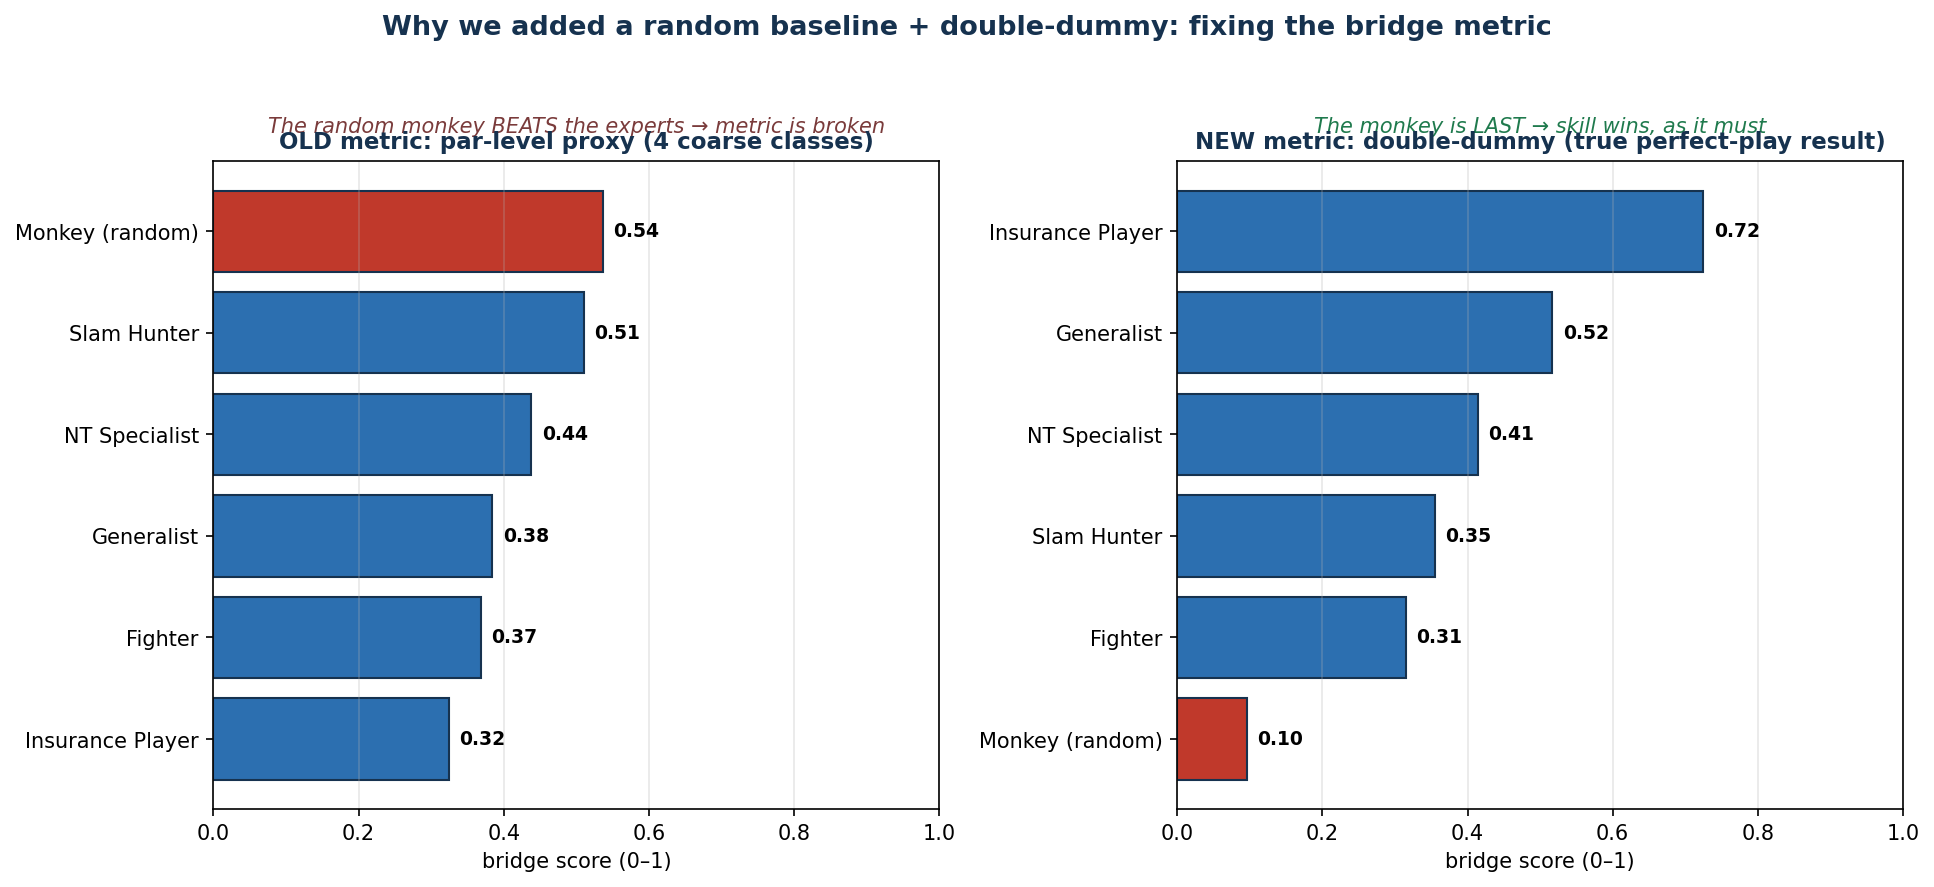
\includegraphics[width=\textwidth]{../docs/images/metric_fix_monkey_dd.png}
\caption{The random baseline exposes (left) and the double-dummy metric fixes
(right) the bridge score.}
\end{figure}

Bridge skill was then measured from the \emph{real} competitive results
(duplicate IMP versus the field, defence included). On this scale the random
monkey sits at $-7$~IMP per board, the elite profiles cluster near $0$, and
double-dummy perfect play marks the ceiling at $+1.1$:

\begin{figure}[H]
\centering
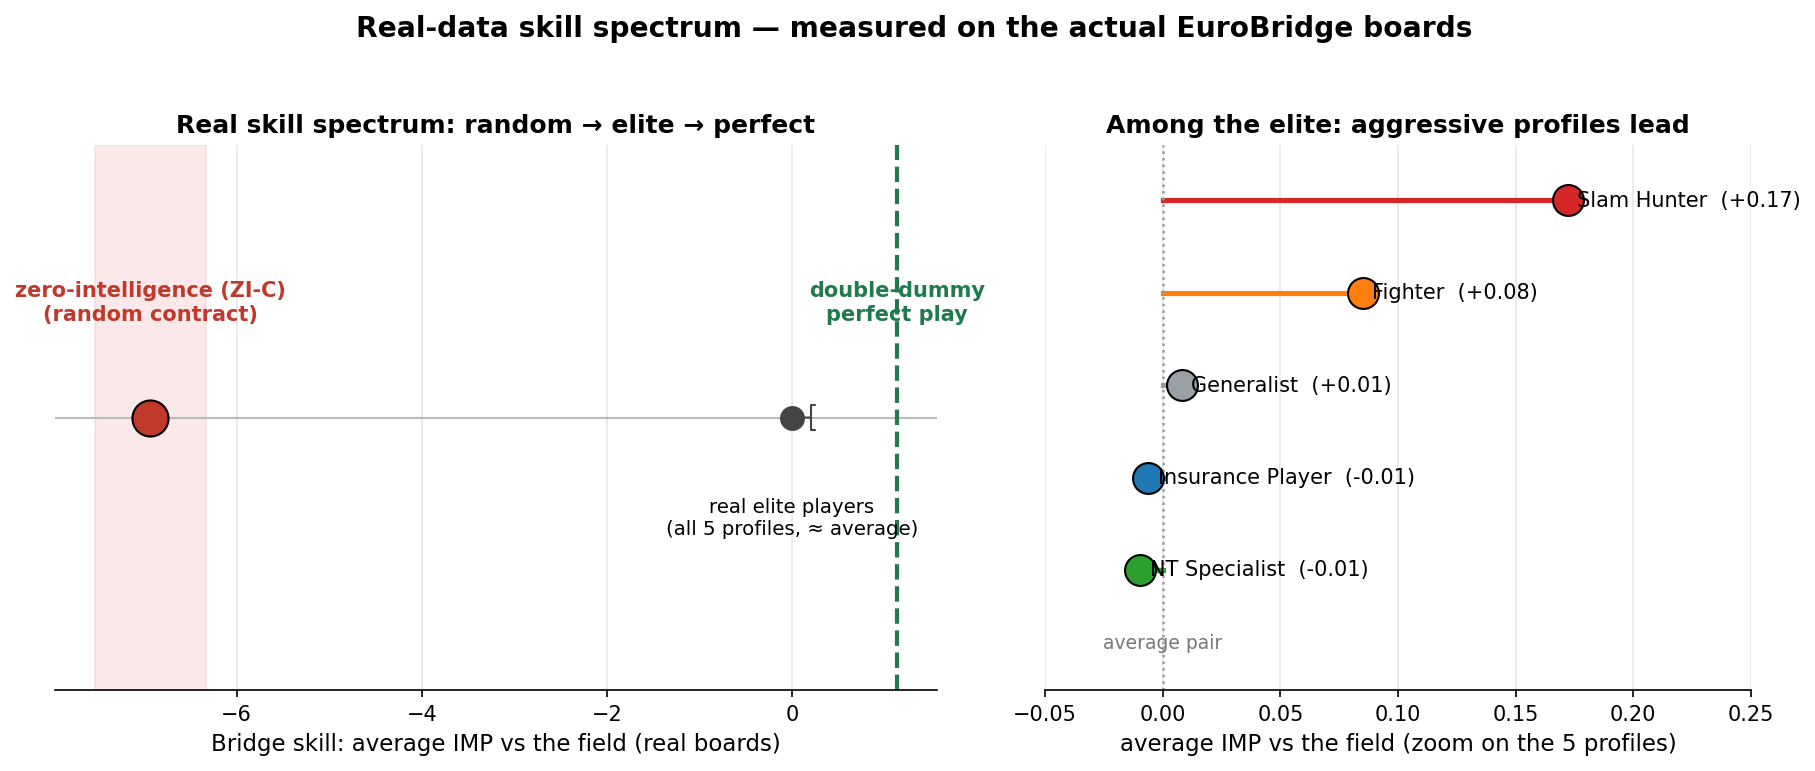
\includegraphics[width=\textwidth]{../docs/images/real_skill_spectrum.png}
\caption{Real-data skill spectrum: random floor $\rightarrow$ elite players
$\rightarrow$ perfect-play ceiling.}
\end{figure}

\section{The discovery: style transfers, winning does not}
Correlating \emph{winning} across domains proved weak and metric-sensitive
($\rho \approx +0.2$ to $+0.5$), because whether a style wins depends on the
opponent and the payoff rules. Refining the question to its original
behavioural form --- does an aggressive bridge profile \emph{bargain}
aggressively? --- yields \textbf{Spearman $\rho = +0.80$}:

\begin{figure}[H]
\centering
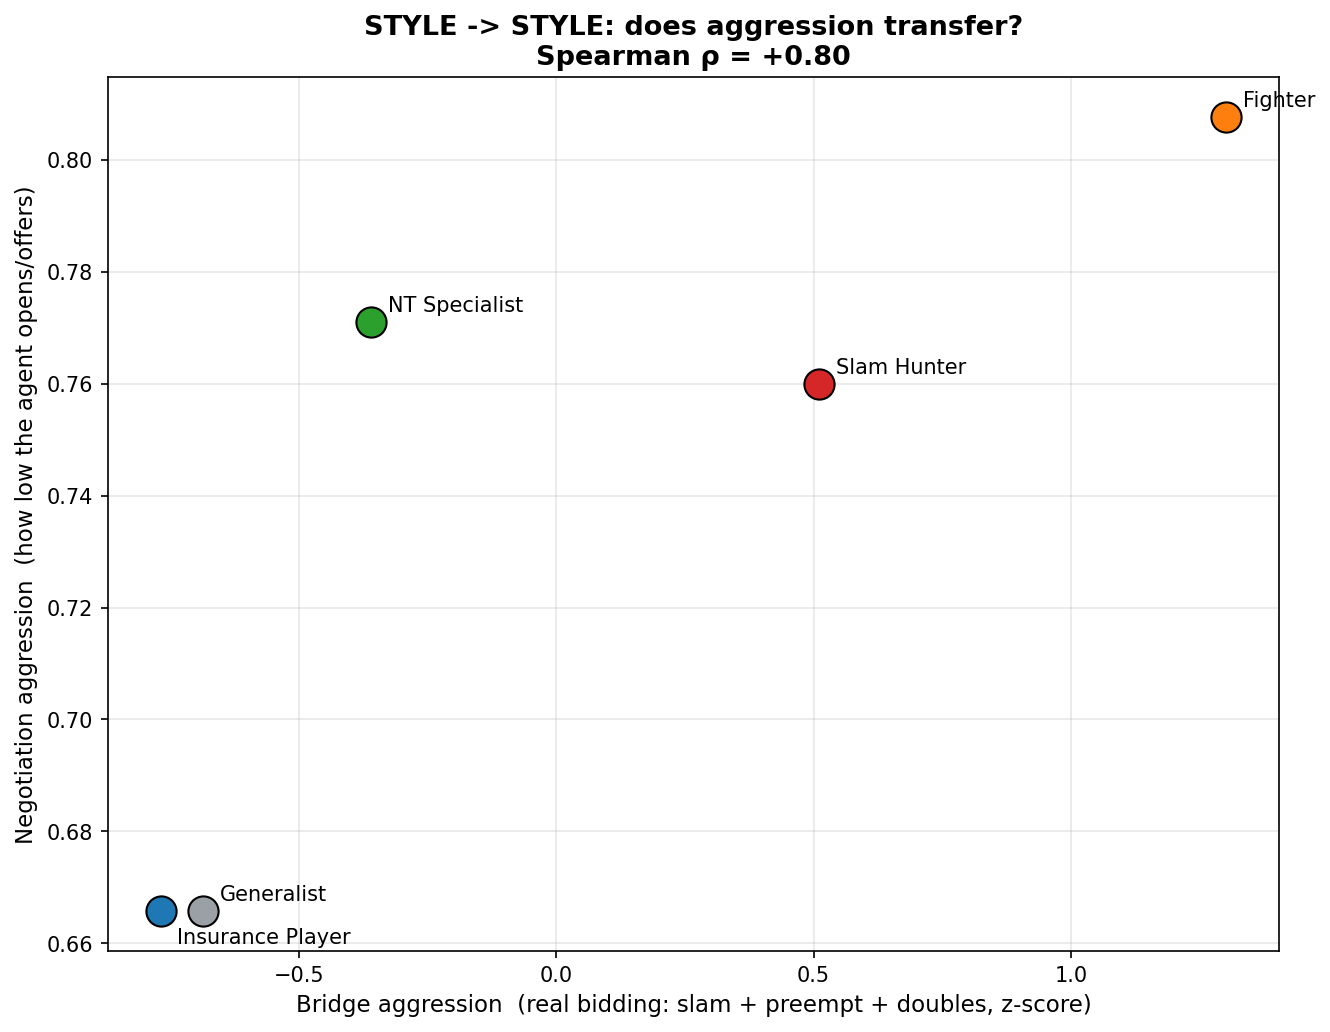
\includegraphics[width=0.78\textwidth]{../docs/images/style_alignment.png}
\caption{Style$\leftrightarrow$style: bridge aggression (real bidding) vs.\
negotiation aggression (how low the agent opens), $\rho = +0.80$.}
\end{figure}

\section{The anti-tautology control}
To rule out ``the agent is aggressive because we labelled it aggressive,''
each profile kept its identity but received the \emph{opposite} profile's
bridge skills. The correlation flipped from $+0.80$ to $\mathbf{-0.90}$
($p = 0.037$) --- behaviour follows the injected bridge-derived skills, not
the label:

\begin{figure}[H]
\centering
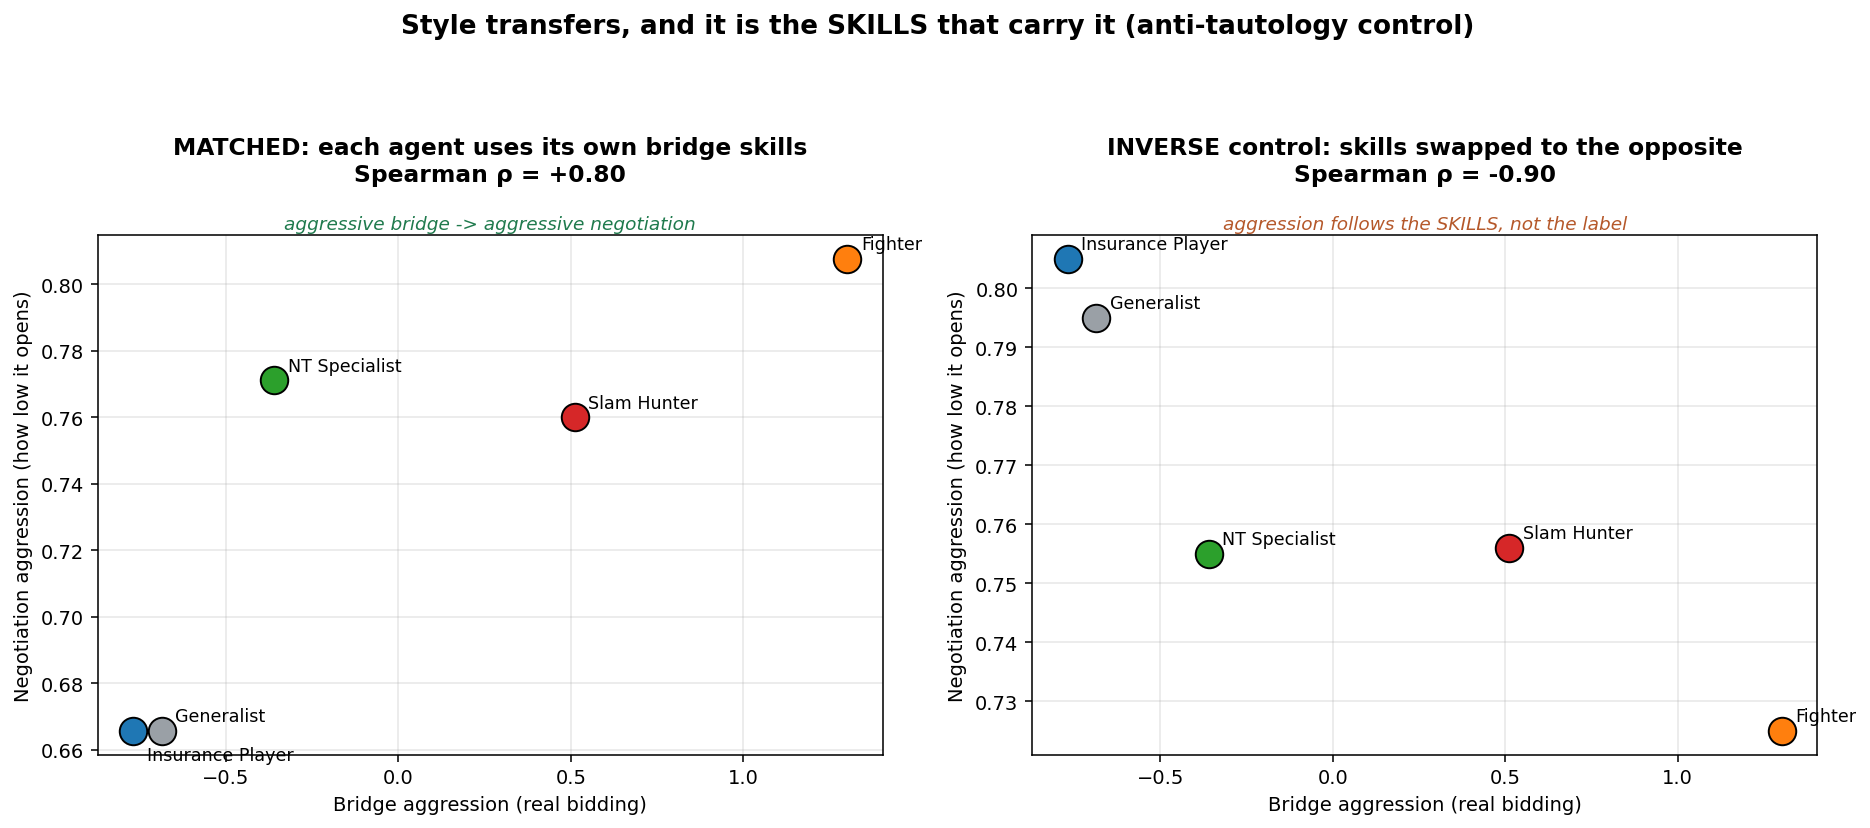
\includegraphics[width=\textwidth]{../docs/images/style_transfer_control.png}
\caption{Matched skills (left, $+0.80$) vs.\ swapped skills (right, $-0.90$):
the skills carry the style.}
\end{figure}

\section{Honest limitations}
With $n = 5$ profiles the style correlation is indicative
($p \approx 0.10$), not significant; negotiation is simulated (calibrated on
real human negotiations, but no same-person negotiation data exists); and the
Slam Hunter profile, defined by \emph{bidding} slams, may partly proxy
overall playing strength. These are documented, not hidden.

\chapter{The AI Layer: LLM Agents and Skill Engineering}
\label{ch:ai}

\section{Agent architecture}
All agents inherit from an abstract \texttt{BaseAgent} that owns the profile
signature, the LLM client, and a single decision choke-point. No agent calls
a provider SDK directly --- every decision flows through one method, which
centralises retries, JSON parsing, temperature policy, and cost logging:

\begin{lstlisting}
class BaseAgent(ABC):
    def _decide(self, user_prompt, response_schema, purpose) -> dict:
        """The ONLY path to the LLM: schema-enforced, logged, retried."""
        response = self.client.generate(
            system=self.system_prompt, user=user_prompt,
            purpose=purpose, temperature=self.temperature,
            response_schema=response_schema)
        return response.json or json.loads(response.text)
\end{lstlisting}

Two concrete agents implement the domains: \texttt{BridgeAgent.make\_bid()}
(temperature $0$ for reproducibility; every returned call is validated by a
local, non-LLM legality checker and falls back to \texttt{Pass} if illegal)
and \texttt{NegotiationAgent.respond\_to\_offer()} (temperature $0.7$;
returns \texttt{counter}/\texttt{accept}/\texttt{walk\_away} with a price
clamped to the scenario's legal range).

\section{Skill extraction and the anti-tautology rule}
Stage 2 turns raw hands into a \emph{skill profile}: hands are chunked
(20--30 per call), sent with a strict JSON schema
(\texttt{response\_mime\_type="application/json"}), and aggregated across
chunks. The cardinal engineering rule: agents are \textbf{never} given
personality adjectives. The Fighter's card says \emph{``doubles opponents at
6--8$\times$ the field rate''} --- a fact extracted from its players' real
auctions --- not \emph{``be aggressive.''} Any cross-domain behaviour must
therefore \emph{emerge} from bridge-derived skills. The inverse-prompt
control (Chapter~\ref{ch:keyresults}) is the executable test of this rule:
swapping the skills swaps the behaviour ($\rho: +0.80 \rightarrow -0.90$).

\section{Prompt engineering as configuration}
Prompts are code-reviewed artefacts, not ad-hoc strings: a central library
(\texttt{shared/prompts.py}) builds every character card from the same
template --- identity line, 5--7 extracted skills, domain rules, a strict
output schema, and a few-shot example. Temperature, schema, and provider are
parameters, so an experiment is a configuration change, not a rewrite.

\section{Engineering against non-determinism}
LLMs are non-deterministic even at temperature $0$ (parallel GPU execution).
The system therefore treats reproducibility at the \emph{sample} level:
every (profile, deal) is run three times with majority voting; every raw
response is persisted to JSONL before aggregation; and all analyses are
recomputable from the persisted artefacts without new API calls. Deals
themselves come from a seeded generator, so the entire experiment replays
bit-identically up to the LLM boundary.

\section{Provider-neutral LLM client}
A single \texttt{LLMClient} wraps Gemini (default), Claude, and OpenAI behind
one interface (an Adapter pattern). It implements exponential-backoff
retries, a per-request 60-second HTTP timeout (a hung socket once stalled a
1{,}500-call batch --- the timeout converts hangs into retryable failures),
and a JSONL cost log per call (provider, model, tokens, latency, USD).
Total project LLM spend: ${\approx}\$1.70$.

\chapter{Software Engineering}
\label{ch:se}

\section{Architecture: a single SDK entry point}
The codebase follows a strict facade discipline: every public operation is
reachable through \texttt{src/sdk.py}, and no function lives only in a
notebook or script. Modules are organised by pipeline stage:

\begin{lstlisting}
src/
  sdk.py                  # facade: the single public contract
  stage1_clustering/      # features, profiling, validation
  stage2_skills/          # chunker, extractor, aggregator
  stage3_agents/          # BaseAgent, BridgeAgent, NegotiationAgent
  stage4_simulate/        # bridge_game, bridge_auction, negotiation,
                          # monkey_agent, alignment
  features/double_dummy.py  # DDS perfect-play evaluator (endplay)
  shared/                 # llm_client, prompts, data_loader, logger
\end{lstlisting}

Design patterns in active use: \textbf{Facade} (\texttt{sdk.py}),
\textbf{Template Method} (\texttt{BaseAgent.\_decide()}),
\textbf{Adapter} (provider-neutral \texttt{LLMClient}),
and \textbf{Strategy} (interchangeable profile agents, including the
\texttt{MonkeyAgent} baseline, which is duck-typed to drop into every runner
unchanged).

\section{Testing}
The project ships $100{+}$ \texttt{pytest} tests: pure-logic units (deal
generation, scoring, auction legality --- 28 tests for the bridge engine
alone), the random-baseline agent (legality of every random call,
reproducibility under a fixed seed), the double-dummy evaluator (known
fixtures: a 12-trick deal must score $6$NT${}=1.0$ and $7$NT${}=0.0$), and
the LLM-dependent layers tested by \emph{injecting a mocked client} --- no
network, no API key, no cost:

\begin{lstlisting}
def test_monkey_bids_are_always_legal_over_many_auctions():
    monkey = MonkeyAgent(seed=1)
    for auction in AUCTION_FIXTURES:
        for _ in range(50):
            out = monkey.make_bid(HAND, auction)
            assert is_legal_call(out["bid"], auction)
\end{lstlisting}

\section{Reliability engineering}
The long simulation runs are engineered to survive real-world failure modes
observed during the project: a per-request HTTP timeout (hangs
$\rightarrow$ retries), per-board \emph{atomic} retry with pauses (rides out
provider 503 load spikes without losing the batch), and incremental JSONL
checkpointing with \texttt{flush()} after every board --- a killed run keeps
all completed work and progress is observable from the file system.

\section{Reproducibility and data discipline}
Fixed seeds (\texttt{random\_state=42}) across scikit-learn and the deal
generator; raw data immutable (\texttt{data/raw} is read-only by
convention); every derived number traceable to a persisted artefact; and the
full history in Git under conventional-commit discipline
(\texttt{feat(stage4): ...}, \texttt{docs(guide): ...}). Every figure in
this portfolio is generated by a committed script --- nothing is hand-drawn,
so documentation cannot drift from the data.

\section{Code quality and cost as an engineering budget}
Style and typing are enforced with \texttt{ruff}, type hints, and
Google-style docstrings on all public functions. LLM cost is treated as an
engineering budget: model selection is empirical
(\texttt{gemini-2.5-flash-lite} proved $10\times$ faster than the default
for this workload), every call is metered, and the complete project ---
all stages, reruns included --- cost ${\approx}\$1.70$.

\chapter{Conclusions and Future Work}

\textbf{Conclusions.} (1)~Elite bridge players form a behavioural continuum,
not clusters; statistically validated profiles live in its extreme tails.
(2)~A skill metric that a random agent can beat is broken --- the
random-baseline test materially changed this project's measurements.
(3)~Decision \emph{style} transfers across domains ($\rho = +0.80$,
non-tautological by an executed inverse-prompt control); \emph{winning} does
not transfer cleanly, because winning is a property of the
(style~$\times$~environment) pair.

\textbf{Future work.} More profiles (finer partitioning of the 563 players)
for statistical power; multi-dimensional negotiation-style measurement
(concession speed, walk-away propensity); cross-model replication
(Claude/GPT); separating style from playing strength; and ultimately real
same-person negotiation data.

% =====================================================================
% PART II — PREPARATORY REPORT (full, included)
% =====================================================================
\part{Preparatory Report}
\addtocontents{toc}{\protect\contentsline{chapter}{\protect\numberline{}Full preparatory report (51 pages): research question, methodology, mathematical foundations, results, schedule, work packages, risk management}{}{}}
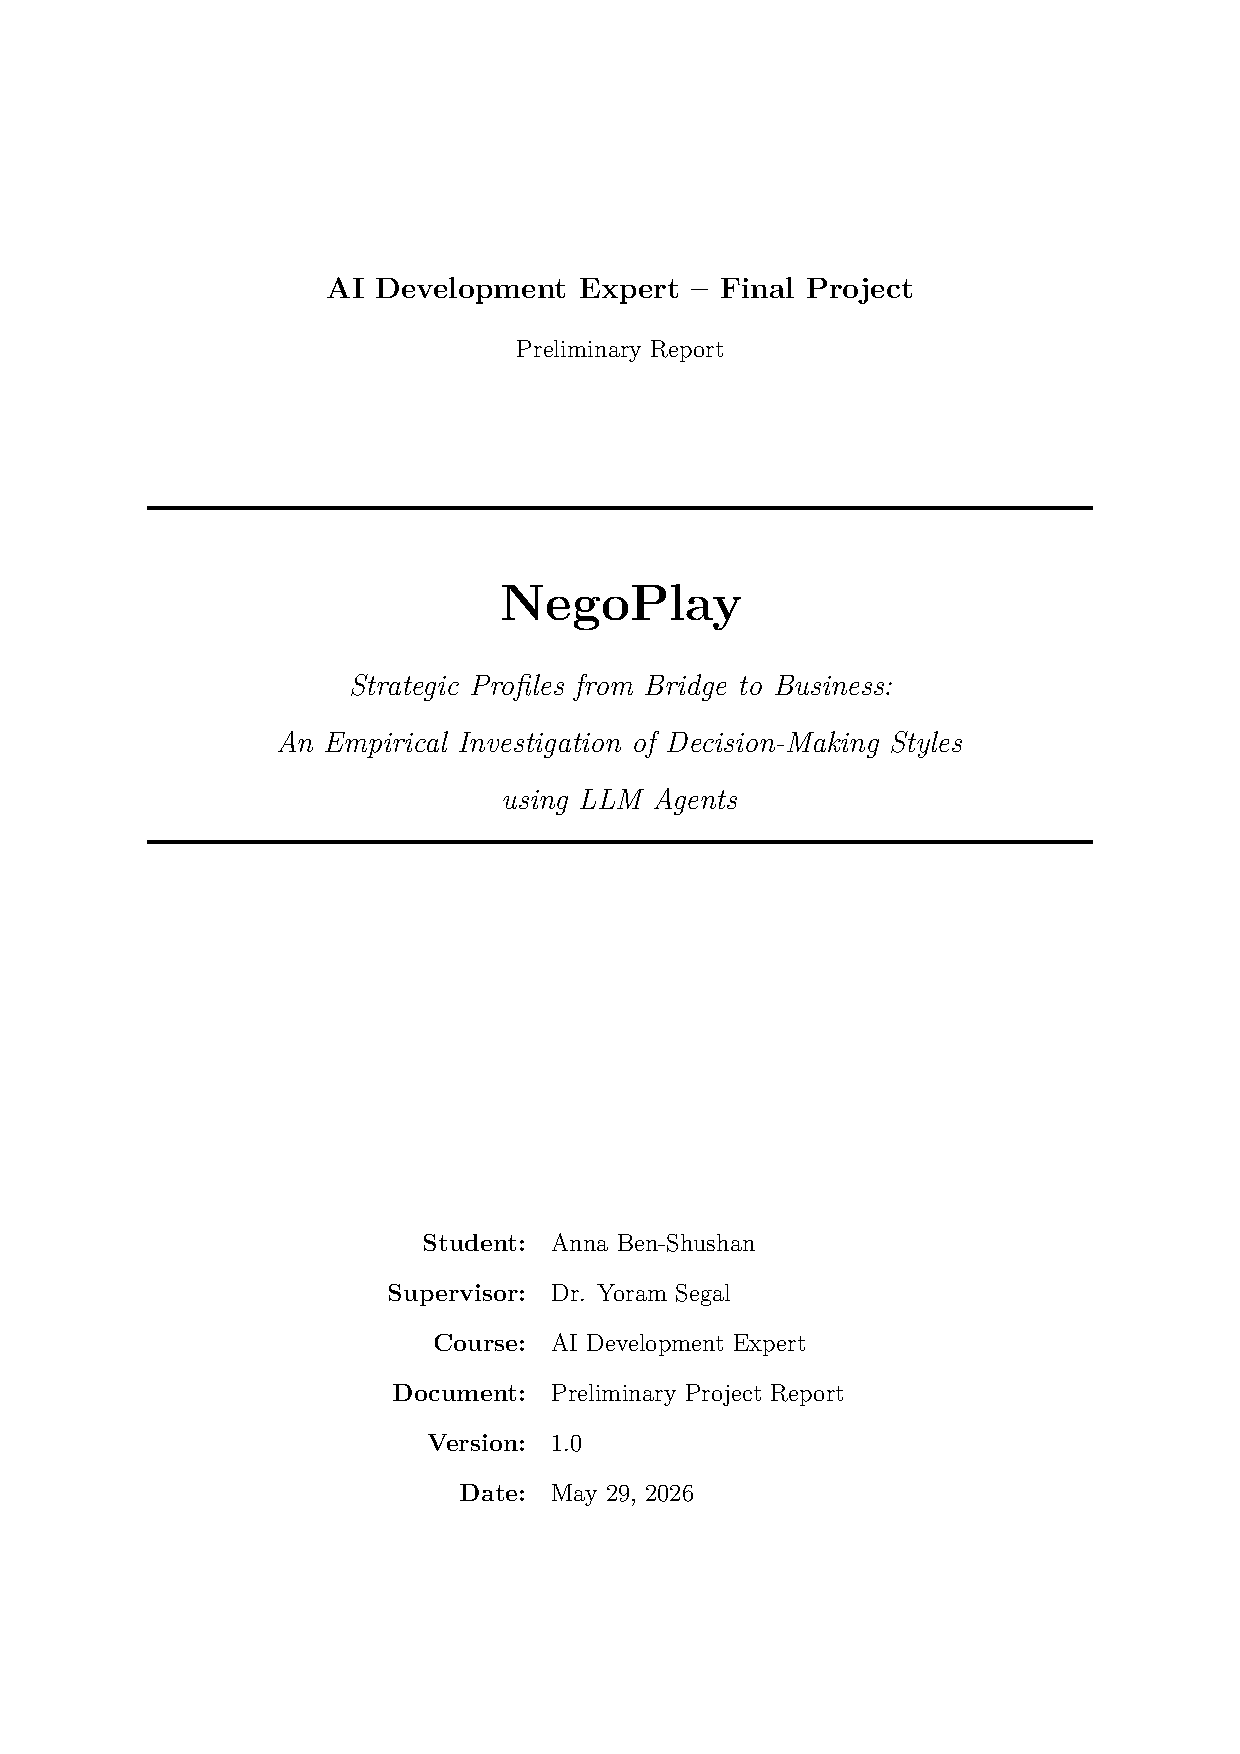
\includepdf[pages=-]{main.pdf}

% =====================================================================
% PART III — BUSINESS PLAN (full, included)
% =====================================================================
\part{Business Plan}
\addtocontents{toc}{\protect\contentsline{chapter}{\protect\numberline{}Full business plan (20 pages): problem, solution, market analysis (TAM/SAM/SOM), business model, token economics, competitive landscape}{}{}}
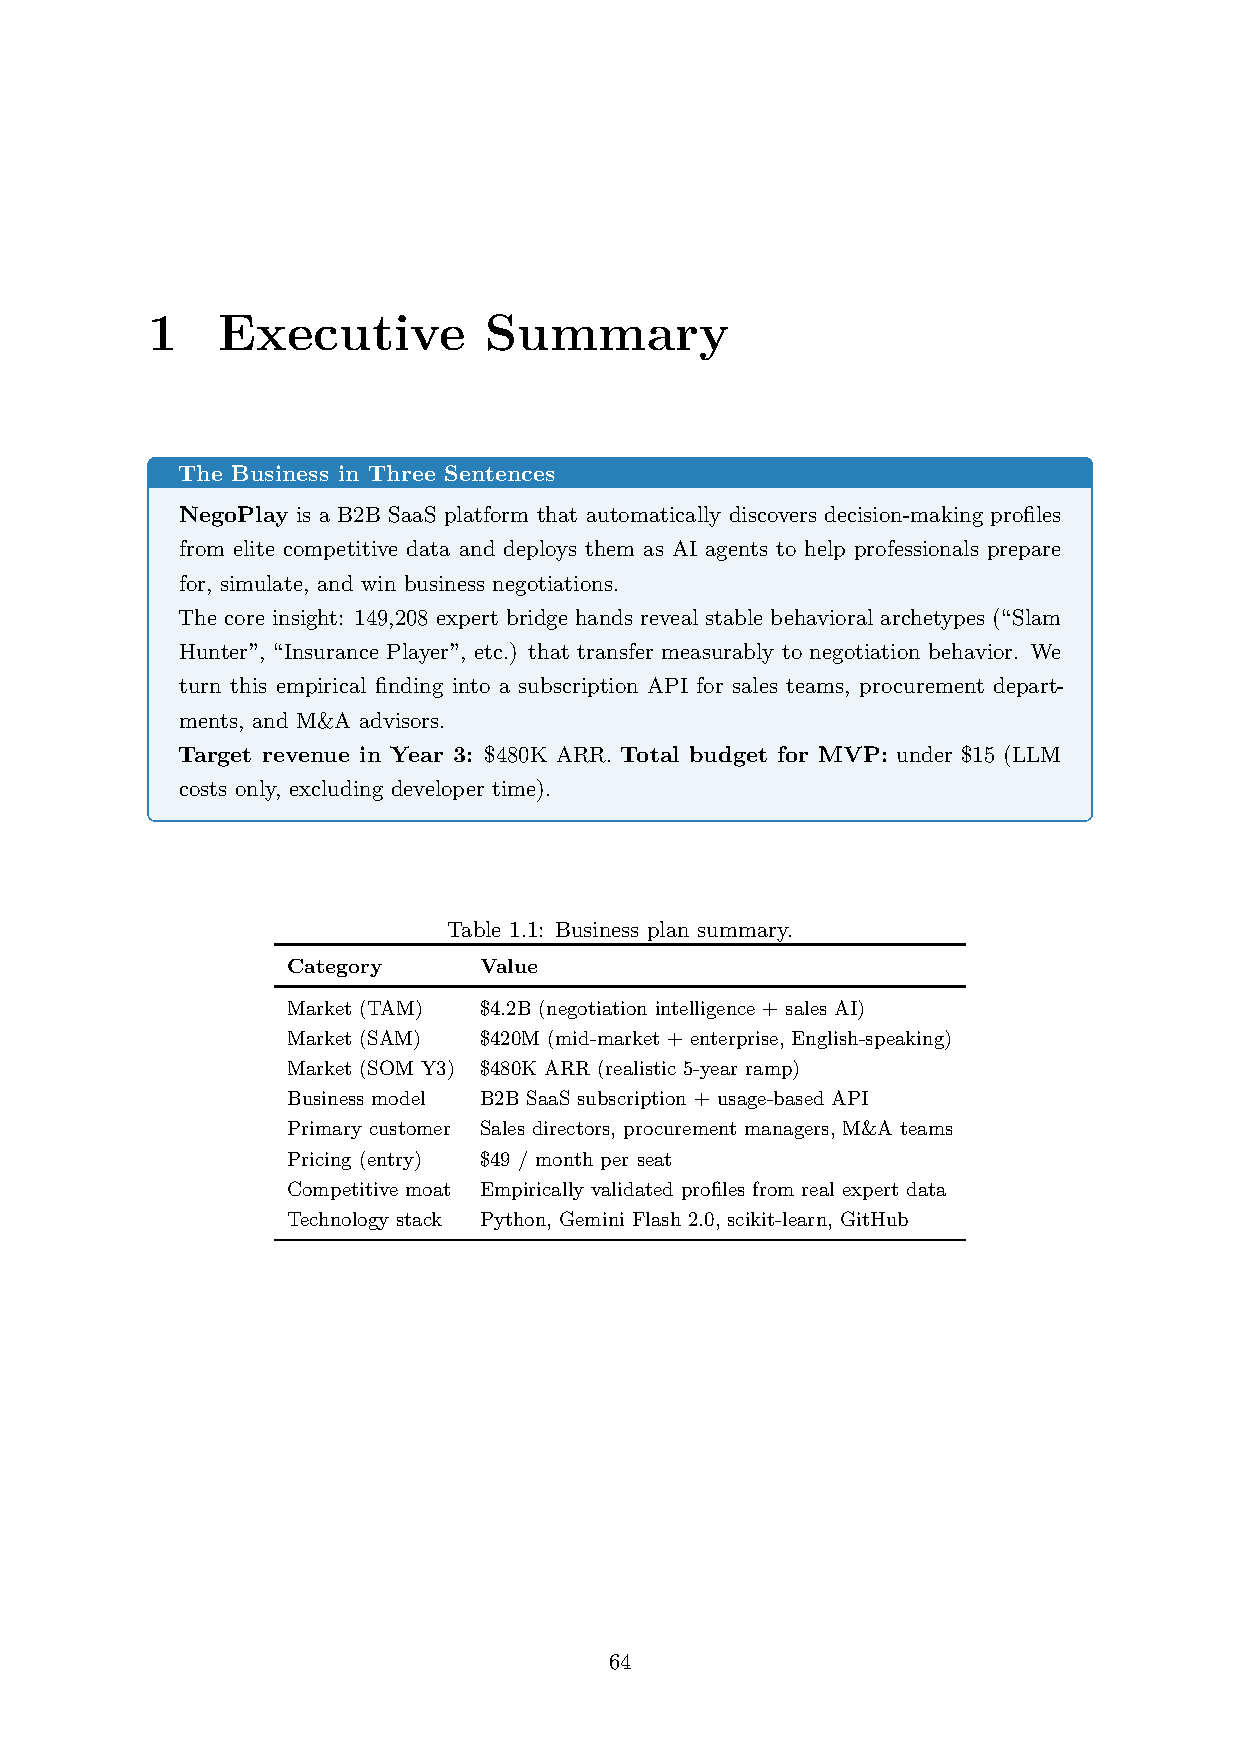
\includepdf[pages=-]{business_plan.pdf}

\end{document}
